\iffalse
This is a big-ish template that I've been using for years now.
A lot of the includes are redundant, so if you're reading this and have no idea why
I've included most things, don't worry - I don't either.
Also, compiling this (to PDF, for instance) relies on CSS files present on my
computer (coming from the packages). So it might not look as nice if you
do it on yours (especially if you don't have all the packages).

Ya'll've been warned.
\fi

\documentclass{article}
    \usepackage{subcaption}
    \usepackage{amsmath}
    \usepackage{amssymb}
    \usepackage{color}
    \usepackage{xcolor}
    \usepackage{graphicx}
    \usepackage{caption}
    \usepackage{float}
    \usepackage[hidelinks]{hyperref}
    \usepackage{enumitem}
    \usepackage[bottom]{footmisc}
    \usepackage{flexisym}
    \usepackage{cancel}
    \usepackage[margin=.8in, tmargin=.8in]{geometry}
    \usepackage{titlesec}
    \usepackage{physics}
    \usepackage{flexisym}
    \usepackage{wrapfig}

    \renewcommand{\baselinestretch}{1.2}
    \newcommand{\eps}{\epsilon}
    \newcommand{\tens}{\otimes}
    \newcommand{\asdef}{\triangleq}
    \newcommand{\w}{\mathbf{w}}
    \newcommand{\x}{\mathbf{x}}
    % \newcommand{\l}{\left(}
    
    
    \setlength\parindent{0pt}
    \captionsetup{justification=centering}
    
    \title{Computer Communications and Networks 2017 Summary}
    \date{\today}
    \author{Traiko Dinev \textless traiko.dinev@gmail.com\textgreater}
    
\begin{document}
\maketitle

\textit{NOTE: Some images were taken from the COMN course (Edinburgh). Everything is publicly accessible via the link at the end of the document. Credit goes to Myungjin Lee (\url{http://homepages.inf.ed.ac.uk/mlee23/}).}

\textit{NOTE: Note this "summary" is NOT a reproduction of the course materials nor is it copied from the corresponding courses. It was entirely written and typeset from scratch.}

\textit{License: Creative Commons public license; See README.md of repository}

\section{Network Layers (Stack)}
Different depending on who you ask. Sometimes contains \textit{Presentation} and \textit{Session} (think cookies) layers. See \url{https://en.wikipedia.org/wiki/OSI_model}

\begin{itemize}
    \item Application layer - messages (\textbf{HTTP}, \textbf{P2P})
    \item Transport layer - segments (\textbf{TCP}, \textbf{UDP})
    \item Network layer - datagrams (\textbf{IP})
    \item Link layer - frames (\textbf{Ethernet})
    \item Physical layers - bits (Check out the Signals summary (TODO))
\end{itemize}

\section{Capacity, delays}

\textit{Bandwidth} $\equiv$ link capacity a.k.a transmission rate ($R\ [\text{bits/s}]$).
\vskip 0.in
Transmissions delay: $L\ [\text{bits}] / R\ [\text{bits/s}]$ for an $L$-bit packet.

\subsection{Transmission}
\begin{itemize}
    \item Store and forward: We store each packet and forward the first one in the queue
    \item Time-division multiplexing: Each receiver gets a slot in time. Slots rotate per a given time.
    \item Frequency-division multiplexing: Same as TDM, but in frequency domain (think Fourier transform)
\end{itemize}

\begin{figure}
    \centering
    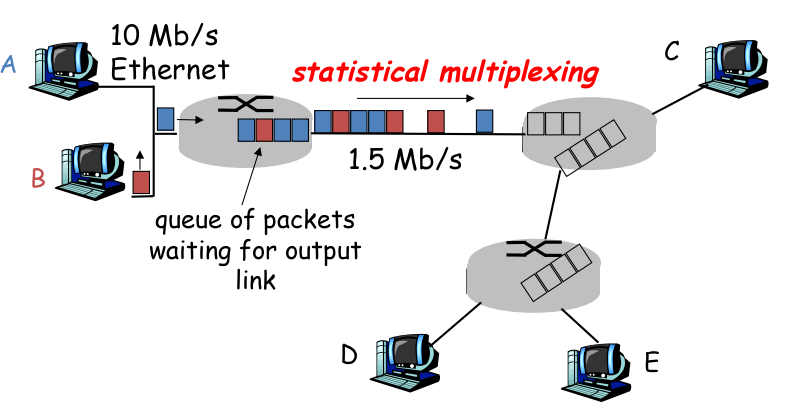
\includegraphics[width=0.7\textwidth]{figures/tdm.png}
    \label{fig:tdm}
    \caption{Time-division multiplexing (from COMN)}
\end{figure}


\subsection{Delays in transmission}
\begin{wrapfigure}{r}{0.5\textwidth}
    \centering
    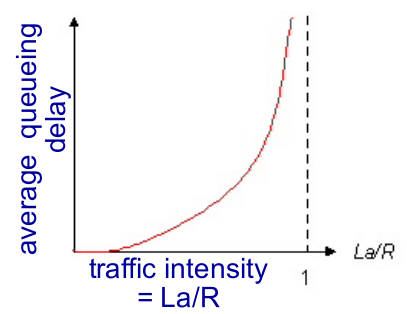
\includegraphics[width=0.5\textwidth]{figures/delay.png}
    \label{fig:tdm}
    \caption{Time-division multiplexing (from COMN)}
\end{wrapfigure}


5 sources of delays
\begin{itemize}
    \item Nodal processing delay
    \item Queuing delay (queue of packets)
    \item Transmission delay (above)
    \item Propagation delay: through the wire, dependent on the speed of light $\frac{d}{s}$, $s\approxeq 3x10^8 m/s$
\end{itemize}

Figure to the right, $a$ is the average arrival of packets, $L$ and $R$ are defined above.

\subsection{Throughput}
Throughput is basically $\frac{\text{transferred data}}{\text{time}}$. The time is usually measured as 
\begin{equation}
    \text{time}\ =\ \text{Round-trip time}\ + \ \frac{\text{size}}{\text{bottleneck BW}}
\end{equation}

\textbf{BW-delay product}: describes the "volume" of the channel (think pipe). Measured in bits/second.

\section{Application layer}
\textbf{HTTP} works over TCP (wiki's fine), sends "resource" requests and receives the resources. Either persistent, where it can receive more than one resource (e.g. page, image, etc.) or non-persistent, where it establishes a new TCP connection for each request (see below). Persistent connections add +1 RTT per request, non-persistent +2 RTT. TCP has a 3-way handshake, hence the persistent one can ask for data on the third packet sent.

HTTP request types, but any can be used for anything:
\begin{itemize}
    \item GET - get resource (common)
    \item POST - update resource (common)
    \item PUT - create new resource 
    \item DELETE - delete resource
\end{itemize}

Status codes:
\begin{itemize}
    \item 200 - OK
    \item 301 - Permanently Moved
    \item 400 - Bad Request
    \item 404 - Not Found
    \item 505 - Version not supported
    \item 500 - Error
\end{itemize}

Cookies are stored in the actual request (via $\text{set-cookie:}$). Example request:

\begin{figure}
    \begin{verbatim}
        GET /index.html HTTP/1.1
        Host: www.website.com
        Accept: image/gif, image/jpeg, */*
        Accept-Language: en-us
        Accept-Encoding: gzip, deflate
        User-Agent: Mozilla/4.0 (compatible; MSIE 6.0; Windows NT 5.1)
        Cookie: MyName = MyValue
        (blank line)
    \end{verbatim}
    \label{fig:http}
    \caption{Example HTTP request}
\end{figure}

\subsection{DNS}
Domain Name Service, Website name $\rightarrow$ IP address.

\begin{itemize}
    \item \textbf{Canonical} names are the most explicit/ longest (www.thisismywebsite.com)
    \item DNS servers store tuples (Name, Values, Type, TTL)
\end{itemize}

DNS Record types are:
\begin{table}[h]
    \centering
    \begin{tabular}{ lll }
        Type & Name & Value \\
        \hline
        \textbf{A} & hostname & IP \\
        \textbf{NS} & domain & authoritative DNS server \\
        \textbf{CNAME} & domain & domain \\
        \textbf{MX} & domain & mail server \\
    \end{tabular}
    \caption{DNS record types}
    \label{tab:dns}
\end{table}

\subsection{Peer-to-peer (P2P)}
Definitions: $F$ - file size. $d_{min}$ - minimum download capacity. $u_s$ - server upload capacity. $u_i$ - download capacity of peer.
\vskip 0.1in

Client-server is one server transmitting files to many clients. P2P is when one person uploads the file (as a server) and then everybody downloads it from each other. The server and the first person is always $u_s$.

Client-server delay until file transmission:
\begin{equation}
    D_{\text{client-server}}\ =\ \text{max}\lbrace \frac{NF}{u_s}, \frac{F}{d_{\text{min}}} \rbrace
\end{equation}

The first term is the total upload size by the server, the second is the slowest download time. P2P delay is bounded:
\begin{equation}
    D_{\text{P2P}}\ \geq\ max \lbrace \frac{F}{u_s}, \frac{F}{d_{\text{min}}}, \frac{NF}{(u_s + \sum_i u_i)} \rbrace
\end{equation}

First term is the upload of the original file, then the max time for one peer to download it and then the sum total of the downloaded size over the sum total of the uploaded size.

\begin{figure}
    \centering
    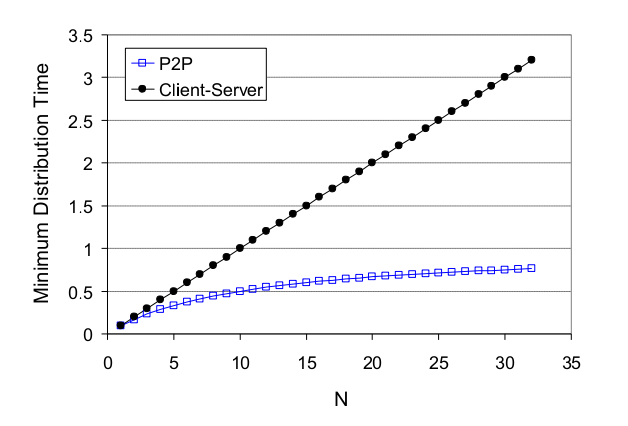
\includegraphics[width=0.7\textwidth]{figures/p2p.png}
    \label{fig:download}
    \caption{P2P vs. Server download times (from COMN)}
\end{figure}

\subsection{Bittorrent}
\begin{itemize}
    \item One tracker has a list of torrents
    \item Torrent is P2P (see above)
    \item Peer churn - peers come and go
    \item Tit-for-tat - every client uploads to top 4 contributors + 1 random one with the hope that the random will become a top.
    \item Optimistically unchoke one peer every 10s (1 above)
\end{itemize}

\subsection{Distributed Hash Table (DHT)}
\begin{itemize}
    \item (key, value) store in peers
    \item Key is converted to integer
    \item Put the key in the closest successor by ID
    \item Circular ordering makes it easier to index or we can have shortcuts to the addresses of peers
\end{itemize}

\section{User Datagram Protocol (UDP)}
\begin{figure}
    \centering
    \begin{subfigure}{0.3\textwidth}
        \centering
        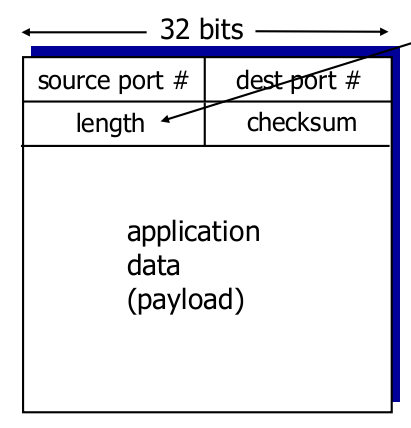
\includegraphics[width=\textwidth]{figures/udp.png}
        \label{fig:udp_header}
        \caption{UDP segment (from COMN)}
    \end{subfigure}
    %
    \centering
    \begin{subfigure}{0.6\textwidth}
        \centering
        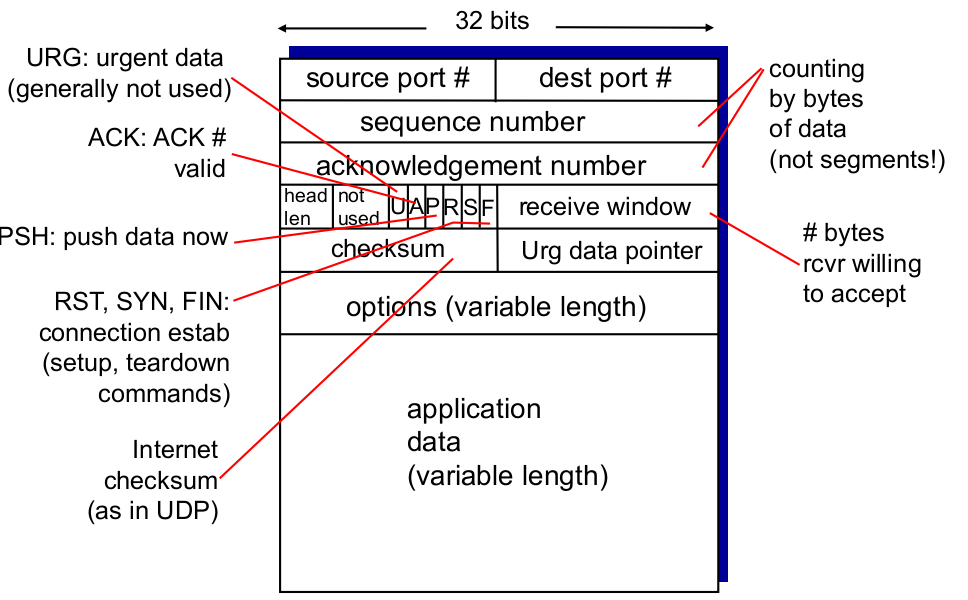
\includegraphics[width=\textwidth]{figures/tcp_header.png}
        \label{fig:tcp_header}
        \caption{TCP segment (from COMN)}
    \end{subfigure}
\end{figure}

\begin{itemize}
    \item Connectionless, just sends packets to destination port
    \item Length is header + data
    \item Checksum is $1^s$ complement of sums of all $16$-bit integers. So read the data as integers, sum and do $1^s$ complement.
\end{itemize}

\section{Transmission Control Protocol (TCP)}
\begin{figure}
    \centering
    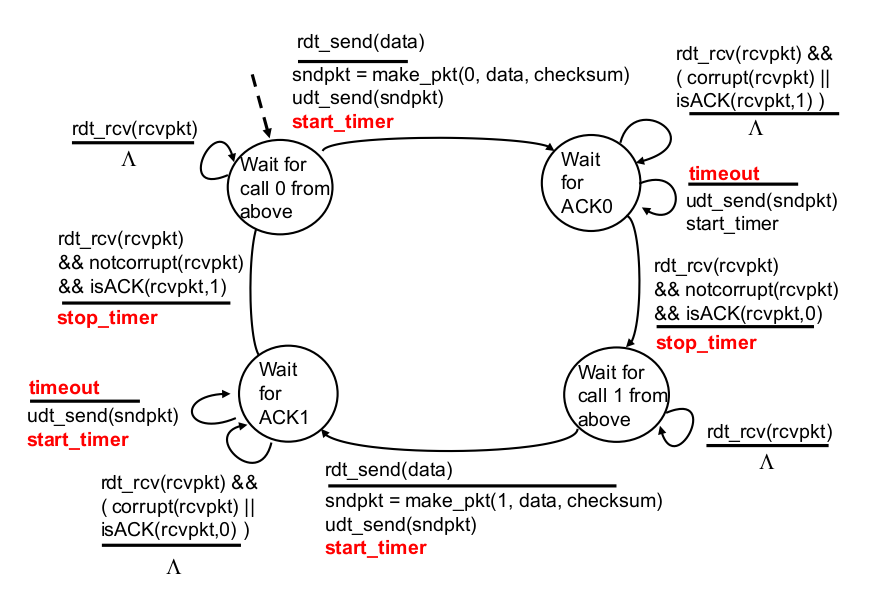
\includegraphics[width=1\textwidth]{figures/tcp.png}
    \caption{TCP (RDT 3.0) reliable transfer sender (kind of complicated) (from COMN)}
    \label{fig:udp}
\end{figure}

A couple of iterations to get there. The following are principles of \textbf{Reliable Data Transfer (RDT)}
\begin{itemize}
    \item \textbf{RDT 1.0} - perfect channel, just use UDP
    \item \textbf{RDT 2.0} - has bit errors, but we can do checksums to detect and send ACK (acknowledgment) and NACK messages for the client to re-send every packet.
    \item \textbf{RDT 2.1} - like 2.0, but ACK can also get garbled. We do sequence numbers for each packet, instead of 1/0 ACK/NACK.
    \item \textbf{TDT 2.2} - just has ACK, which is cumulative, so up to the last received packet
    \item \textbf{3.0} - 2.2 but with timeout for lost packets. Basically TCP.
\end{itemize}

\vskip 0.1in
\textbf{Stop and Wait} - sends one packet and waits for response.
\vskip 0.03in\textbf{Go-back-N} - Wait for cumulative ACKs, otherwise resend previous N packets.
\vskip 0.03in
\textbf{Selective Repeat} - Sliding window of packets, send repeat for each packet not received (timeout).

Check this for a cool visualization \url{http://www.ccs-labs.org/teaching/rn/animations/gbn_sr/}.
TCP is Go-back-n (GBN). Speeds are:
\begin{align}
    D_{\text{transmission}}\ &=\ \frac{L}{R} \\
    U_{\text{sender}}\ &=\ \frac{\frac{N\ L}{R}}{\frac{L}{R}\ +\ \text{RTT}}
\end{align}

\subsection{Actual TCP}
See figure \ref{fig:tcp_conns} for the TCP handshake/connect and disconnect.

\begin{figure}
    \centering
    \begin{subfigure}{0.3\textwidth}
        \centering
        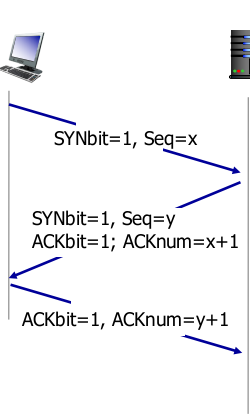
\includegraphics[width=\textwidth]{figures/tcp_open.png}
        \label{fig:tcp_open}
        \caption{TCP connect (from COMN)}
    \end{subfigure}
    \hspace{20mm}
    \begin{subfigure}{0.55\textwidth}
        \raggedright
        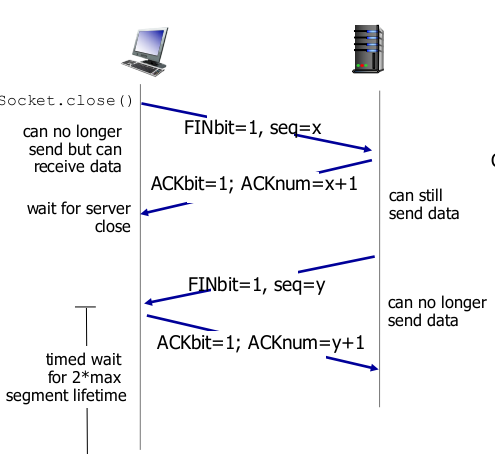
\includegraphics[width=\textwidth]{figures/tcp_close.png}
        \label{fig:tcp_close}
        \caption{TCP close (from COMN)}
    \end{subfigure}
    \caption{TCP connections}
    \label{fig:tcp_conns}
\end{figure}

\subsubsection{Flow Control}
Do not overwhelm receiver by keeping track of their buffer (GBN):
\begin{align*}
    \text{RTT}\ &=\ (1\ -\ \alpha)\ \text{Estimated}\ +\ \alpha\ \text{SampleRTT} \\
    \text{DevRTT}\ &=\ (1\ -\ \beta)\ \text{DevRTT}\ +\ \beta\ \left|\text{SampleRTT}\ -\ \text{EstimatedRTT}\right| \\
    \text{Timeout}\ &=\ \text{EstimatedRTT}\ +\ 4\ \text{DevRTT}
\end{align*}

Read Kurose and Ross about this, it's kind of complicated. Otherwise check figure \ref{fig:tcp_flow_control}. For the difference between Tahoe and Reno check out figure \ref{fig:tahoe_reno}.


\begin{figure}
    \centering
    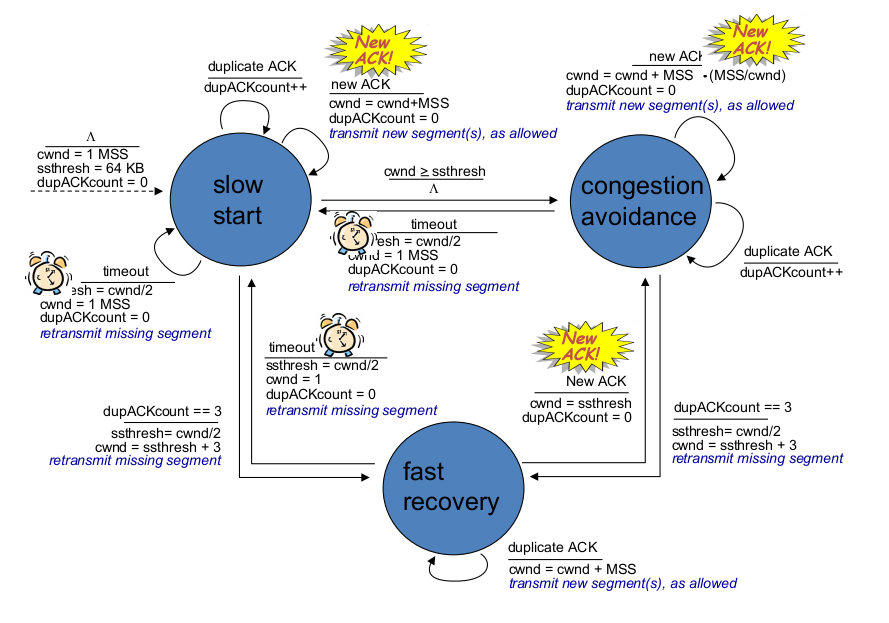
\includegraphics[width=1\textwidth]{figures/flow_control.png}
    \caption{TCP Flow Control (kind of complicated) (from COMN)}
    \label{fig:tcp_flow_control}
\end{figure}

\begin{figure}
    \centering
    \begin{subfigure}{0.49\textwidth}
        \centering
        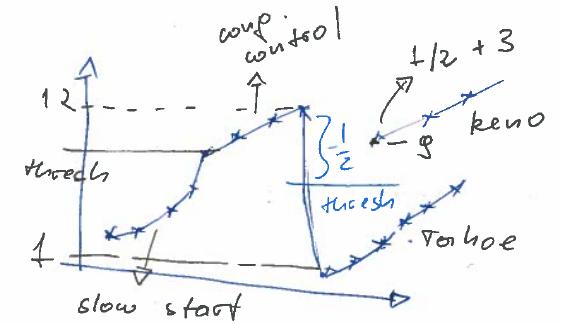
\includegraphics[width=1\textwidth]{figures/tahoe_reno.png}
        \caption{TCP Reno vs Tahoe (original work :D)}
        \label{fig:tahoe_reno}
    \end{subfigure}
    % \hspace{20mm}
    \begin{subfigure}{0.49\textwidth}
        \raggedright
        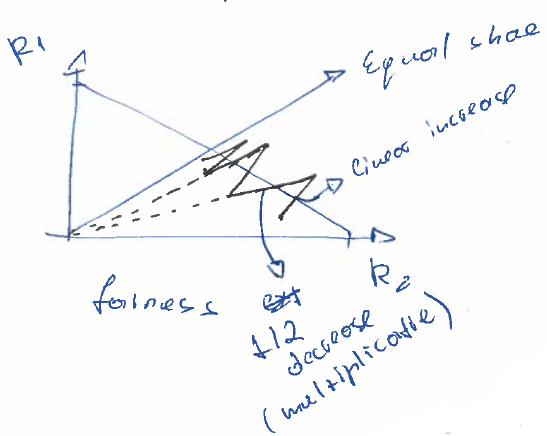
\includegraphics[width=1\textwidth]{figures/fairness.png}
        \caption{TCP Fairness (original work)}
        \label{fig:fairness}
    \end{subfigure}
    \caption{TCP flow/ congestion control}
    \label{fig:tcp_fairness_congestion}
\end{figure}

Fairness is in figure \ref{fig:fairness}. In the beginning (slow start) CWND increases by 1 MSS (Maximum Segment Size)for both connections. This means they increase along a 45 degree line. Once the bandwidth becomes too high, they both halve it, meaning it's now halfway towards the origin. And so on.

\section{Network Layer}
\subsection{Routers}
Longest prefix matching in a table, routes to physical links connected to the router. 
\begin{table}[h]
    \centering
    \begin{tabular}{ lll }
        IP Range & Link \\
        \hline
        192.168.1.x & 0 \\
        15.*.*.* & 1 \\
        otherwise & 2
    \end{tabular}
    \caption{DNS record types}
    \label{tab:router}
\end{table}

\textbf{IP Mask}: 192.168.0.32/24 bits means the mask is 192.168.0.x

\begin{itemize}
    \item \textbf{CIDR} - classless interdomain routing (masks)
    \item \textbf{Subnet} - machines in it can communicate without routers
    \item \textbf{DHCP} - protocol for obtaining IP addresses
    \begin{itemize}
        \item MSG type discover $\rightarrow$ sent to 255.255.255.255 (broadcast)
        \item MSG with leased IP is sent back to 255.255.255.255 (see Ethernet below)
    \end{itemize}
    \item \textbf{ICANN} - Internet Corporation for Assigned Names and Numbers (for DNS)
    \item \textbf{NAT} - Network Address Translation: Routers at the Network Layer bind connections to the outside to $\text{IP}_{\text{out}}$/$\text{PORT}_{\text{out}}$ to a local port \textbf{on the router}. Connections are then routed to that computer.
    \begin{itemize}
        \item \textbf{DMZ} (Demilitarized Zone) - when one computer is exposed to the outside behind the router
    \end{itemize}
    \item \textbf{ICMP} - Internet Control Message Protocol
    \begin{itemize}
        \item Used to send signals via IP (i.e. without TCP or UDP on top)
        \item Type 0, Code 0 $\rightarrow$ echo, ping
        \item Type 11, Code 0 $\rightarrow$ TTL expired, used for $traceroute$
    \end{itemize}
    \item \textbf{IPv6}
    \begin{itemize}
        \item $40$ byte header, $128$ bit IP
        \item no checksums
        \item \textbf{ICMPv6} has more control messages
        \item \textbf{IPv4} datagram can contain \textbf{IPv6} messages, meaning we can use v6 with v4 routers, so long as the \textbf{IPv6} routers are aware of the v4 protocol
    \end{itemize}
\end{itemize}

The following are algorithms to route between routers.
\subsection{Dijkstra}
\begin{itemize}
    \item $c(x, y)$ $\rightarrow$ cost from $x$ to $y$
    \item $D(v)$ $\rightarrow$ cost of path to $v$
    \item $P(v)$ $\rightarrow$ predecessor node
    \item $N$ $\rightarrow$ visited node
\end{itemize}

Then just google Dijkstra..
\subsection{Bellman-Ford}
Uses this equation:
\begin{equation}
    d_x(y)\ =\ \text{min}_v \{ c(x, v)\ +\ d_v(y) \}
\end{equation}

Here $d_x(y) \rightarrow$ distance from x to y. We need to keep track of all the neighbors' distance vectors ($D_v\ =\ [D_v(y): y\ \in\ N]$). They get synchronized every so often. The vectors are basically tables, computed with the equation above. If we iterate, then it eventually computes the correct values.
\vskip 0.1in
We have AS (autonomous systems). Think a collection of routers, usually in the same subnet. Some of the protocols are Inter-AS (between ASes, ha-ha..), some Intra-AS (inside Ases, um..).

\subsection{Routing Information Protocol (RIP)}
\textit{IntraAS}
\begin{itemize}
    \item Uses Bellman Ford (a.k.a Distance Vector)
    \item 30sec. advertisement from every router
    \item if something is 16 hops away, then it's $\infty$
    \item 180sec. = dead link
    \item uses UDP
\end{itemize}

\subsection{OSPF - Open Shortest Path First}
\textit{IntraAS}
\begin{itemize}
    \item Open source, uses Dijkstra
    \item Advertisement flooded to entire AS (autonomous system)
    \item Customizable security 
\end{itemize}

\subsection{BGP - Border Gateway Protocol}
\textit{InterAS}
\begin{itemize}
    \item over semi-permanent TCP connections
    \item see illustration (figure \ref{fig:bgp})
    \begin{itemize}
        \item Once a subnet (the outside world) becomes reachable
        \item The router advertises it and puts itself as the next hop
        \item AS-Path is the path taken to reach the target subnet
        \item And so routers know where to send packets to reach the subnet (71.0.0.0/8 in the diagram)
    \end{itemize}
\end{itemize}

\begin{figure}
    \centering
    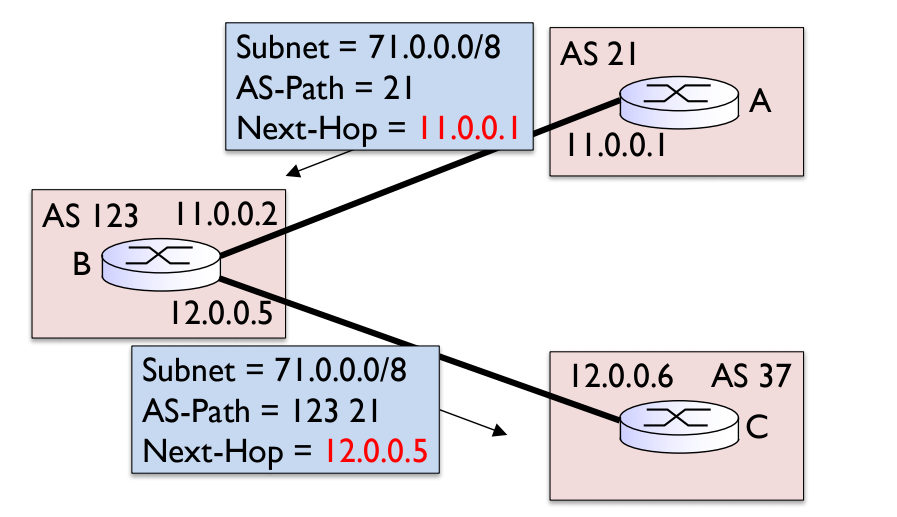
\includegraphics[width=1\textwidth]{figures/bgp.png}
    \caption{BGP operation (from COMN)}
    \label{fig:bgp}
\end{figure}

\section{Link Layer}
This is mostly low-level communication without knowledge about IPs. It's sending packets over physical Wires. See the scanned figures \ref{fig:scanned} for the details.

\begin{itemize}
    \item \textbf{Time division multiple access}: each machine gets a time slot
    \item \textbf{FDMA}: Same with frequencies, uses Fourier transform to accomplish it
    \item \textbf{Slotted Aloha} - Each node transmits in slots. If there is a collision, then the node retransmits the frame in each subsequent slot with prob p until it succeeds.
    \begin{itemize}
        \item The efficiency is $Np(1-p)^{N-1}$, i.e. each node must be the only one transmitting, where p is the probability of a node sending a frame and N is the number of nodes.
    \end{itemize}
    \item \textbf{Unslotted Aloha} - Each node just transmits when it needs to. Need to consider the time interval $[t_0 - 1, t_0]$, $[t_0, t_0 + 1]$ for analysis.
    \begin{itemize}
        \item The efficiency is $P(\text{success}) = P(\text{node transmits})\ P(\text{no other in} [t_0 - 1, t_0]) P(\text{no other in} [t_0, t_0 + 1])$, which is $p (1 - p)^{N -1} ( 1 - p)^{N - 1}$, which is even worse than the slotted version.
    \end{itemize}
\end{itemize}


\begin{figure}
    \centering
    \begin{subfigure}{0.8\textwidth}
        \centering
        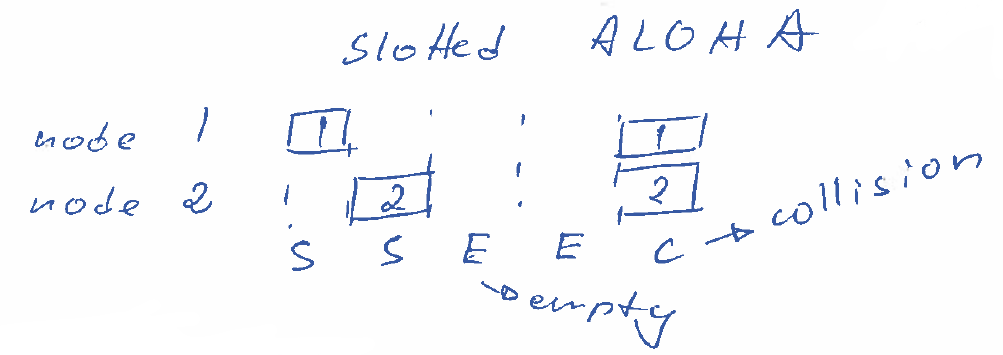
\includegraphics[width=1\textwidth]{figures/slotted_aloha.png}
        \caption{Slotted Aloha}
        \label{fig:slotted_aloha}
    \end{subfigure}
    \vskip 0.6in
    \begin{subfigure}{0.45\textwidth}
        \raggedright
        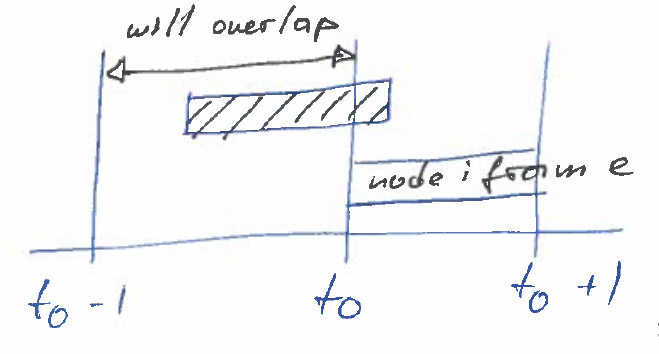
\includegraphics[width=1\textwidth]{figures/unslotted_aloha.png}
        \caption{Unslotted Aloha}
        \label{fig:unslotted_aloha}
    \end{subfigure}
    \hspace{10mm}
    \begin{subfigure}{0.45\textwidth}
        \raggedright
        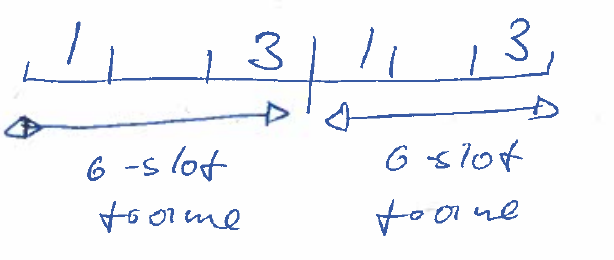
\includegraphics[width=1\textwidth]{figures/tdma.png}
        \caption{TDMA}
        \label{fig:tdma}
    \end{subfigure}
    \caption{Transmission protocols}
    \label{fig:scanned}
\end{figure}

\subsection{Carrier Sense Multiple Access (CSMA)}
Used by Wi-Fi mostly, see figure \ref{fig:csma}. Once a node detects a collision, it does Binary exponential back-off. This means each node chooses a delay at random from the set $\{ 0, 1, ..., 2^{m - 1}\}$ to wait. Efficiency is:
\begin{equation}
    \frac{1}{1 + \frac{5\ t_{\text{prop}}}{t_{\text{trans}}}}
\end{equation}

\begin{figure}
    \centering
    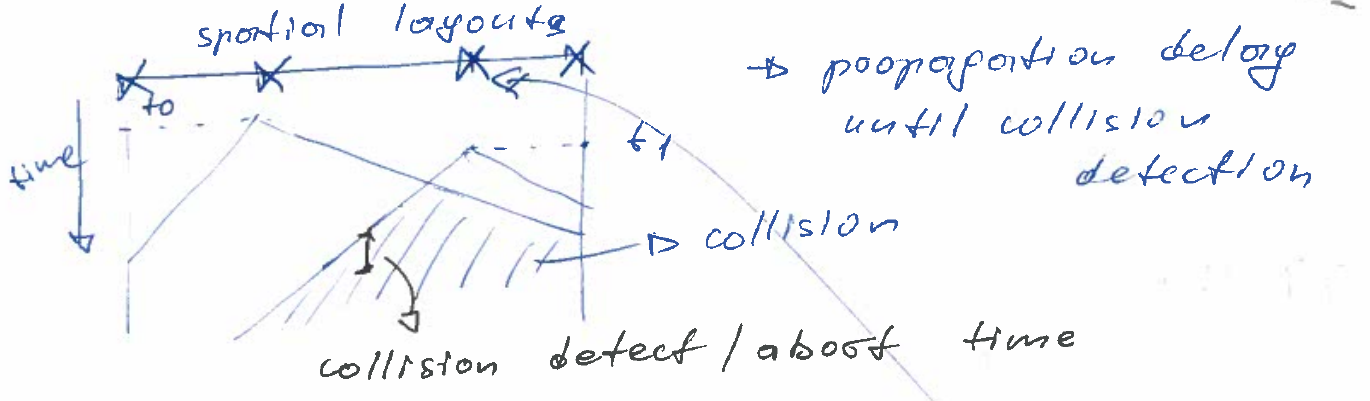
\includegraphics[width=1\textwidth]{figures/csma.png}
    \caption{CSMA. The crosses are routers (say, Wi-Fi) in space. The signal propagates through time and collisions are detected by the router with some delay.}
    \label{fig:csma}
\end{figure}

\subsection{Address Resolution Protocol (ARP)}
This translates IP addresses to MAC (Media Access Control) addresses, which Ethernet (below) uses for communication. Has a table of IP to MAC addresses.

\begin{table}[h]
    \centering
    \begin{tabular}{ lll }
        IP & Mac \\
        \hline
        192.168.123.1 & 11:22:33:44:55:AA \\
    \end{tabular}
    \caption{ARP Records}
    \label{tab:dns}
\end{table}

\subsection{Ethernet}
See figure \ref{fig:ethernet}. Low level communication based on MAC addresses. Uses Cyclic Redundancy Codes for error correction.

\begin{figure}
    \centering
    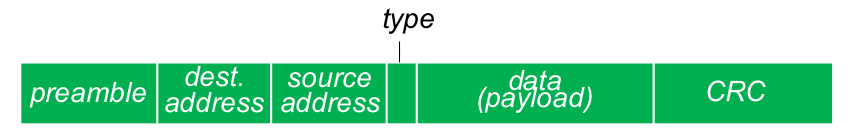
\includegraphics[width=1\textwidth]{figures/ethernet.png}
    \caption{Ethernet Frame.}
    \label{fig:ethernet}
\end{figure}

\section{Overview}
Here's an overview of the entire procedure of opening a webpage. Inspired by Kurose and Ross' Retrospective: A Day in the Life of a Web Page. I \textbf{highly recommend} you read that as well, since it's much more detailed and puts everything together nicely.

\begin{itemize}
    \item \textit{Scenario}: We want to open Google
    \item First, we need an IP. We create a \textbf{DHCP} request, put it in a \textbf{UDP} segment that goes into an \textbf{IP} datagram which goes into a \textbf{Ethernet} frame. The destination IP address is broadcast ($255.255.255.255$) and so is the destination MAC address (FF:FF:FF:FF:FF).
    \item The router gets the frame, demultiplexes it back up to \textbf{DHCP} and allocates some IP with a lease. Then that is sent back via a \textbf{DHCP} ACK message back to broadcast.
    \item The router also put its address ($192.168.0.1$) as a default gateway, so that requests first go there.
    \item \textbf{DNS}: We now need google's IP. We create a DNS query via UDP that has a destination IP as obtained from the DHCP request.
    \item The frame needs to go to the gateway, but we do not know its MAC address. We create an \textbf{ARP} query with the target IP of the gateway ($192.168.0.1$). The Ethernet frame this goes in still has a broadcast address (FF:FF:FF:FF:FF:FF).
    \item The router sends back the \textbf{ARP} reply with its MAC address (BB:BB:BB:BB:BB).
    \item We send the DNS query with the \textbf{DNS}'s server IP ($8.8.8.8$), but the Ethernet frame is addressed to the gateway router (BB:BB:BB:BB:BB).
    \item \textbf{OSPF, BGP, etc.} protocols used by the routers tell them where to forward the DNS frame, which bounces around and goes back to our computer.
    \item \textbf{TCP} We create a TCP request to Google's IP and the rest is easy.
\end{itemize}

\section{FAQ}
\begin{itemize}
    \item Why use MAC \textit{and} IP addresses?
    \begin{itemize}
        \item MAC addresses are hard-coded into network cards. They were the old way of communicating. IP came afterwards and groups things together (think subnets). Hence it works on top of Ethernet as described above.
    \end{itemize}

    \item What happens to MAC addresses between router hops?
    \begin{itemize}
        \item They get overridden. When you go through a router, it will put its interface MAC as the source MAC, since it's the only machine reachable from the outside.
    \end{itemize}

    \item Can you describe this better?
    \begin{itemize}
        \item Check this out
        
        \textit{
        Bit late but still here is my answer :) ... To send data you need two address, the MAC address and the IP address. Basically the sending host will ARP for a MAC address, this occurs when the local host doesn't know the MAC address of the host it has an IP address for or it will ARP for the default gateway MAC address (if it doesn't already know it) if the IP address in on a different subnet/ network. Once it obtains a MAC address the IP packet is encapsulated in a L2 frame and sent across the media. If the IP packet is meant for a host on a different subnet/ network, it will be sent to the default gateway, this router will de-encapsulate the L2 frame (remove and discard it) check the IP address and will forward it. For the router to do this it needs a MAC address to send it over the media, It will look up the next hop in it's routing table, encapsulate the IP packet with the same source and destination IP address that was sent from the original host into a new L2 frame. This time the MAC address for the source address will be that of the forwarding interface of the router, and the receiving interface of the next hop will be the destination MAC address. This will continue from hop to hop until it reaches the final host, each time the MAC addresses will change, but the original IP address will remain the same.}
    \end{itemize}
\end{itemize}

Last paragraph taken from \\
\url{https://stackoverflow.com/questions/23935095/how-are-mac-addresses-used-in-routing-packets}.


\section{References and Links}
\begin{itemize}
    \item \url{https://www.inf.ed.ac.uk/teaching/courses/comn/} - Edinburgh course on computer networks. What most of this note is based on.
    \item Jim Kurose, Computer Networking: A Top-Down Approach
\end{itemize}

\end{document}
